%Fiquemos com Deus e Nossa Senhora!
%Sao Jose de Cupertino rogai por nos que recorremos a vos!!!
%Honra teu Pai e tua Mãe!
% ### Uses XeLaTeX ### %
% ### Needs beamer-master ### %
\documentclass[aspectratio=169]{beamer} %. Aspect Ratio 16:9

\usetheme{AI2} % beamerthemeSprace.sty
\usepackage{algpseudocodex}
\usepackage[portuguese]{babel}
\usepackage[utf8]{inputenc}
\usepackage[T1]{fontenc}
\usepackage{ragged2e,gensymb,bm,amsmath,amssymb}

\DeclareMathOperator*{\argmin}{arg\,min}
\DeclareMathOperator*{\argmax}{arg\,max}
\DeclareMathOperator{\sign}{sgn}

% DATA FOR FOOTER
\date{2021}
\title{- ISOMAP}
\institute{Advanced Institute for Artificial Intelligence (AI2)}

\begin{document}
% ####################################
% FIRST SLIDE 						:: \SliTit{This is the Title of the Talk}{A. B. Name}{Sprace}
% SUB-TITLE SLIDE 					:: \SliSubTit{<title>}{<explanation}
% SUB-SUB-TITLE SLIDE				:: \SliSubSubTit{<title>}{<explanation}
% SLIDE WITH TITLE 					:: \SliT{Title}{Content}
% SLIDE NO TITLE 						:: \Sli{Content} 
% SLIDE DOUBLE COLUMN WITH TITLE 	:: \SliDT{Title}{First Column}{Second Column}
% SLIDE DOUBLE COLUMN NO TITLE 		:: \SliD{First Column}{Second Column}
% SLIDE ADVANCED WITH TITLE 			:: \SliAdvT{Title}{Content}
% SLIDE ADVANCED NO TITLE 			:: \SliAdv{Content}
% SLIDE ADVANCED DOUBLE WITH TITLE 	:: \SliAdvDT{Title}{First Column}{Second Column}
% SLIDE ADVANCED DOUBLE NO TITLE 	:: \SliAdvD{First Column}{Second Column}
% SLIDE BLACK						:: \Black{ <Content> }
% SLIDE WHITE						:: \White{ <Content> }
% ITEMIZATION 						:: \begin{itemize}  \iOn{First} \iTw {Second} \iTh{Third} \end{itemize}
% COMMENT TEXT				 		:: \note{<comment>}
% SECTION 							:: \secx{Section} | \secxx{Sub-Section}
% BOLD SPRACE COLOR				:: \bfs{<text>}
% TABLE OF CONTENT					:: \tocitem{<title>}{<content>}
% LEFT ALIGN EQUATION				:: \begin{flalign*}  & <equation> &   \end{flalign*}
% CENTER ALIGN EQUATION	S			:: \begin{gather*} <equations>  \end{gather*}
% SLASH								:: \slashed{<>}
% BAR								:: \barr{<letter>} instead of \bar{<letter>}
% THEREFORE						:: use \portanto (larger and bold}
% 2 or 3 MATH SYMBOLS				:: \overset{<up>}{<down>} &  \underset{<below>}{\overset{<above>}{<middle>}}  
% INSERT TEXT IN FORMULA			:: \ins{<text>}
% EXERCISE							:: \exe{<exercise #>}{<exercise text>}
% SUGGESTED READING BOX			:: \sug{<references>}
% CITATION							:: \cittex{<citation>}
% CITATION DOUBLE COLUMN 			:: \cittexD{<citation>}
% TEXT POSITION						:: \texpos{<Xcm>}{<Ycm>}{<text>} origin = center of slide : x right | y down
% REFERENCE AT BOTTOM  S/D SLIDE		:: \refbotS{<reference>} \refbotD{<reference>}
% HIDDEN SLIDE						:: \hid
% COLOR BOX 						:: \blu{blue} + \red{rec} + \yel{yellow} + \gre{green} + \bege{beige}
% FRAME 							:: \fra{sprace} \frab{blue} \frar{red} + \fray{yellow} + \frag{green}		
% FIGURE 							:: \img{X}{Y}{<scale>}{Figure.png} 
% FIGURE							:: \includegraphics[scale=<scale>]{Figures/.png}
% FIGURE DOUBLE SLIDE NO TITLE		::  \img{-4}{0.5}{<scale>}{Figure.png} % Image 1st half
%									::  \img{4}{0.5}{<scale>}{Figure.png} % Image 2nd half
% FIGURE DOUBLE SLIDE WITH TITLE		::  \img{-4}{0}{<scale>}{Figure.png} % Image 1st half
%									::  \img{4}{0}{<scale>}{Figure.png} % Image 2nd half
% INCLUDING SWF (Flash)				:: \usepackage{media9} and \includemedia >> USE ACROBAT <<
%%%%%%%%%%%%%%%%%%%%%%%%%%%%%%%%%%%%%%%%%%%%%%%%%%
% ###############################################################################
% FIRST SLIDE
\SliTit{{\LARGE ISOMAP}}{Advanced Institute for Artificial Intelligence -- AI2}{https://advancedinstitute.ai}
%%%%%%%%%%%%%%%%%%%%%%%%%%%%%%%%%%%%%%%%%%%%%%%%%%
% ###############################################################################
% SLIDE SUB-TITLE
%\SliSubTit{Sub-Title}{Description}{}
%%%%%%%%%%%%%%%%%%%%%%%%%%%%%%%%%%%%%%%%%%%%%%%%%%
% ###############################################################################
%\SliSubSubTit{Sub-Sub-Title}{Description}
 %%%%%%%%%%%%%%%%%%%%%%%%%%%%%%%%%%%%%%%%%%%%%%%%%%


\SliT{Introdução}{

\justifying A técnica \emph{Isometric Feature Mapping} (ISOMAP) é um algoritmo para redução não linear de dimensionalidade que baseia-se no arcabouço de \textbf{aprendizado de variedades} (\emph{manifold} learning). A principal diferença desse método para outros do tipo PCA (KPCA) e LDA/MDA (KFDA) é que aqui construimos uma relação de adjacência entre as  amostras.
}

\Sli{
\justifying \underline{Ideia geral}: construir um grafo unindo os vizinhos mais próximos, calcular os menores caminhos entre cada par de vértices e encontrar um mapeamento para o plano que preserve essas distâncias.

\justifying \underline{Hipótese}: caminhos mínimos em um grafo podem aproximar bem as distâncias geodésicas em espaços não Euclidianos (variedades).

\justifying \underline{Aprendizado de métricas}: métodos lineares falham em aprender uma medida de distância adequada na presença de não linearidades nos dados.

\begin{center}
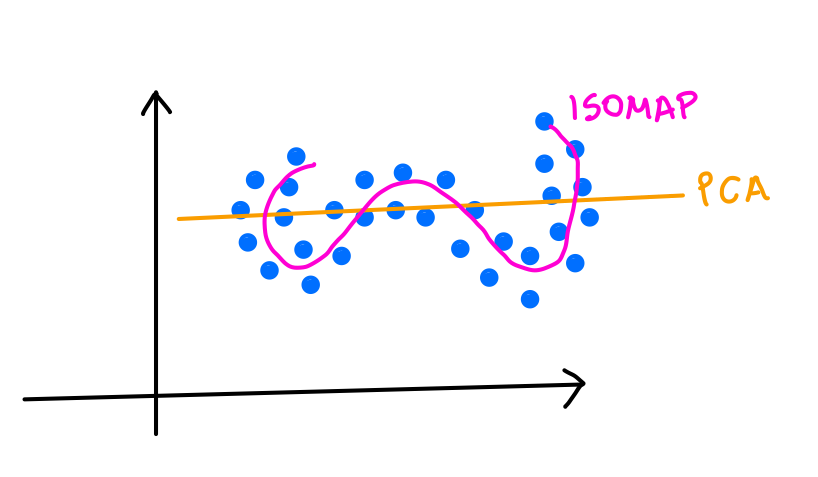
\includegraphics[scale=0.23]{./figs/ISOMAP_Fig1.png}
\end{center}
}

\Sli{
\justifying O algoritmo do ISOMAP pode ser resumidos em três passos:

\begin{enumerate}
	\item Induzir o grafo $k$-nn a partir do conjunto de dados ${\cal X} = \{(\bm{x}_1,y_1),(\bm{x}_2,y_2,\ldots,(\bm{x}_m,y_m)\}$, em que $\bm{x}_i\in\mathbb{R}^n$ e $y\in{\cal Y}$ tal que ${\cal Y}=\{\omega_1,\omega_2,\ldots,\omega_c\}$ e $k<m$.
	\item Criar a matriz de distâncias ponto a ponto $\bm{D}\in\mathbb{R}^{m\times m}$ entre as amostras de ${\cal X}$. Desta forma, $D_{ij}$ representa o menor caminho entre as amostras $\bm{x}_i$ e $\bm{x}_j$.
	\item Encontrar o conjunto de pontos $\hat{{\cal X}}$ no espaço $\mathbb{R}^k$ tal que as distâncias originais sejam "preservadas". Esta etapa é realizada pela técnica MDS (\emph{Multidimensional Scaling}).
\end{enumerate}
Trata-se, portanto, de uma abordagem \textbf{global}, pois utiliza todas as amostras para calcular as distâncias. A técnica é baseada em um teorema que diz que caminhos mínimos em grafos $k$-nn são boas aproximações para as distâncias geodésicas (distâncias que respeitam as variedades).
}

\Sli{
}

\Sli{
\justifying Como podemos calcular essas distâncias geodésicas? Seja ${\cal G}=({\cal V},{\cal E},w)$ um grafo tal que ${\cal V}=\{\bm{v}_1,\bm{v}_2,\ldots,\bm{v}_m\}$ e ${\cal E}$ representam os conjuntos de vértices e arestas, respectivamente, e $w:{\cal V}\times{\cal V}\rightarrow\mathbb{R}^+$ uma função que calcula a distância entre dois nós. Note que os nós do grafos são compostos pelas amostras em ${\cal X}$, ou seja, $\bm{v}_i=\bm{x}_i$.

\justifying Temos que um caminho $P^\ast_{\bm{v}_1,\bm{v}_m}$ é dito ser ótimo se o seu custo $C$ é o menor possível, ou seja:

\begin{equation}
	C(P^\ast_{\bm{v}_1,\bm{v}_m}) = \sum_{i=1}^{m-1}w(\bm{v}_i,\bm{v}_{i+1}) = w(\bm{v}_2,\bm{v}_{2})+w(\bm{v}_2,\bm{v}_{3})+\ldots+w(\bm{v}_{n-1},\bm{v}_{m}), 
\end{equation}
em que $C(P^\ast_{\bm{v}_1,\bm{v}_m})$ se aproxima da distância geodésica entre $\bm{v}_1$ e $\bm{v}_m$.
}

\Sli{
\justifying Uma técnica bastante conhecida para calcular caminhos mínimos em grafos é chamada de \textbf{Algoritmo de Dijkstra}. Existe um teorema que mostra que este algoritmo sempre calcula a distância geodésica entre um nó \textbf{fonte} e demais nós do grafo. A única restrição é quVejamos as seguinte definições:

\begin{itemize}
	\item $\lambda(\bm{v})$: menor custo até o momento de alguma amostra $\bm{s}$ até $\bm{v}$.
	\item $\pi(\bm{v})$: predecessor de $\bm{v}$ no caminho de custo ótimo.
	\item ${\cal Q}$: fila de prioridades dos vértices.
\end{itemize}

}

\Sli{
Vejamos, agora, o algoritmo do Dijkstra. 
\begin{center}
\begin{minipage}{0.4\textwidth}
\begin{algorithmic}
\State \Call{Dijkstra}{${\cal G}$, $\bm{s}$}
	\For{each $\bm{v}\in{\cal V}$}
	\State{$\lambda(\bm{v})\leftarrow+\infty$}
	\State{$\pi(\bm{v})\leftarrow nil$}
	\EndFor
	\State{$\lambda(\bm{s})\leftarrow0$}
	\State{$\pi(\bm{s})\leftarrow nil$}
	\State{${\cal Q}\leftarrow{\cal V}$, ${\cal S}\leftarrow\emptyset$}
	\While{${\cal Q}\neq\emptyset$}
	\State{$\bm{u}\leftarrow Remove({\cal Q})$}
	\State{${\cal S}\leftarrow{\cal S}\cup\bm{u}$}
	\For{each $\bm{v}\in{\cal N}(\bm{u})$}
	\If{$\lambda(\bm{v})>\lambda(\bm{u})+w(\bm{u},\bm{v})$}
	\State{$\lambda(\bm{v})\leftarrow\lambda(\bm{u})+w(\bm{u},\bm{v})$}
	\State{$\pi(\bm{v})\leftarrow\bm{u}$}
	\EndIf
	\EndFor
	\EndWhile
\end{algorithmic}
\end{minipage}
\begin{minipage}{0.42\textwidth}
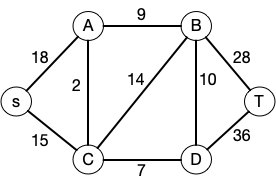
\includegraphics[scale=0.57]{./figs/ISOMAP_Fig2.png}
\end{minipage}%%% to prevent a space
\end{center}
}

\SliT{Multidimensional Scaling}{
\justifying Como fazemos o mapeamento para o espaço $\mathbb{R}^k$ ($k$ é escolhido pelo usuário)? Assim, dada a nossa matriz de distâncias geodésicas calculadas pelo algoritmo de Dijkstra, o objetivo é encontrar um novo mapeamento das amostras de tal forma que suas distâncias originais sejam preservadas. A solução para este problema é dada pela técnica MDS.
\justifying Lembrando que a distância $D_{ij}$ entre dois vetores $\bm{x}_i$ e $\bm{x}_j$ é dada por:

\begin{equation}
	D_{ij} = \norm{\bm{x}_i-\bm{x}_j}^2=(\bm{x}_i-\bm{x}_j)^T(\bm{x}_i-\bm{x}_j).
\end{equation}
Note que a matriz de distâncias $\bm{D}$ já foi calculada anteriormente.
}

\Sli{
\justifying O método MDS baseia-se na solução de dois subproblemas:

\begin{itemize}
	\item Encontrar a matriz $\bm{B}\in\mathbb{R}^{m\times m}$ a partir de $\bm{D}$ e
	\item Recuperar (mapear) as coordenadas dos novos pontos a partir de $\bm{B}$.
\end{itemize}
\justifying Note que $\bm{B}$ corresponde à matriz de produtos internos entre todas as amostras, ou seja, $B_{ij} = \bm{x}_i^T\bm{x}_j$. Vejamos, então, como resolver cada um dos subproblemas.
}

\Sli{
\justifying \underline{Subproblema 1}: encontrar $\bm{B}$ a partir de $\bm{D}$.\newline

\underline{Hipótese}: a média $\bm{\mu}\in\mathbb{R}^n$ dos dados é nula, ou seja:

\begin{equation}
	\bm{\mu} = \frac{1}{m}\sum_{i=1}^m\bm{x}_i = 0.
\end{equation}
Assumimos essa hipótese pois, caso contrário, teremos infinitas soluções para o problema (diferentes versões do espaço que estão transladadas, por exemplo). Ademais, aplicando a operação distributiva na Equação 2, temos que:

\begin{equation}
	D_{ij} = \bm{x}_i^T\bm{x}_i-2\bm{x}_i\bm{x}_j+\bm{x}_j^T\bm{x}_j.
\end{equation}
}

\Sli{
\justifying A partir da matriz $\bm{D}$, podemos calcular a média de uma coluna $s$ da seguinte maneira:
\vspace{-0.3cm}
\begin{align}\nonumber
	M_s &= \frac{1}{m}\sum_{i=1}^mD_{is} = \frac{1}{m}\sum_{i=1}^m\overbrace{(\bm{x}_i^T\bm{x}_i-2\bm{x}_i\bm{x}_s+\bm{x}_s^T\bm{x}_s)}^{D_{is}} = \\
	&= \frac{1}{m}\left(\sum_{i=1}^m\bm{x}_i^T\bm{x}_i-2\sum_{i=1}^m\bm{x}_i\bm{x}_s+\sum_{i=1}^m\bm{x}_s^T\bm{x}_s\right)\\\nonumber
	&= \frac{1}{m}\sum_{i=1}^m\bm{x}_i^T\bm{x}_i-\frac{2}{m}\sum_{i=1}^m\bm{x}_i\bm{x}_s+\frac{1}{m}\sum_{i=1}^m\bm{x}_s^T\bm{x}_s\\\nonumber
	&= \frac{1}{m}\sum_{i=1}^m\bm{x}_i^T\bm{x}_i-2\bm{x}_s\cancelto{0\text{ Equação 3}}{\frac{1}{m}\sum_{i=1}^m\bm{x}_i}+\frac{1}{m}\sum_{i=1}^m\bm{x}_s^T\bm{x}_s\\\nonumber
	&= \frac{1}{m}\sum_{i=1}^m\bm{x}_i^T\bm{x}_i+\frac{1}{m}\sum_{i=1}^m\bm{x}_s^T\bm{x}_s = \frac{1}{m}\sum_{i=1}^m\left(\bm{x}_i^T\bm{x}_i+\bm{x}_s^T\bm{x}_s\right).
\end{align}
}


\Sli{
\justifying Um agradecimento especial ao \textbf{Prof. Alexandre Levada} do Centro de Ciências Exatas e de Tecnologia, Departamento de Computação, Universidade Federal de São Carlos, pelas notas de aula.
}

\end{document}